\documentclass{article}
\usepackage{amsmath}
\usepackage{amssymb} % Required for \mathbb{}
\usepackage[a4paper,margin=0.8in]{geometry}
\usepackage{enumerate}
\usepackage{graphicx}


\begin{document}

\title{Quizz 4 - Optimization}
\author{BCC325 - Intelligência Artificial}
\date{}

\maketitle

\section*{Questão 1}

Para qual das seguintes opções você sempre encontrará a mesma solução, mesmo se executar o algoritmo várias vezes?

Considere um problema em que o objetivo é minimizar uma função de custo e cada estado no espaço de estados tem um custo diferente.

\begin{enumerate}[a)]
    \item Subida de encosta (hill-climbing) com escolha do passo mais íngreme, começando de um estado inicial diferente a cada vez.
    \item Subida de encosta com escolha do passo mais íngreme, sempre começando do mesmo estado inicial.
    \item Subida de encosta estocástica, começando de um estado inicial diferente a cada vez.
    \item Subida de encosta estocástica, sempre começando do mesmo estado inicial.
    \item Tanto a subida de encosta com passo mais íngreme quanto a estocástica, desde que sempre comecem do mesmo estado inicial.
    \item Tanto a subida de encosta com passo mais íngreme quanto a estocástica, começando de um estado inicial diferente a cada vez.
    \item Nenhuma versão da subida de encosta garantirá a mesma solução sempre.
\end{enumerate}



\section*{Questão 2}

Considere o seguinte problema de otimização:

\textit{Um fazendeiro deseja plantar duas culturas, Cultura 1 e Cultura 2, e quer maximizar seus lucros. O fazendeiro obterá um lucro de R\$500 por acre plantado da Cultura 1 e R\$400 por acre plantado da Cultura 2.}

\textit{No entanto, ele precisa fazer todo o plantio hoje, durante as 12 horas entre 7h e 19h. O plantio de um acre da Cultura 1 leva 3 horas, e o plantio de um acre da Cultura 2 leva 2 horas.}

\textit{O fazendeiro também tem uma limitação de suprimentos: ele tem material suficiente para plantar até 10 acres da Cultura 1 e até 4 acres da Cultura 2.}

\textit{Assuma que a variável \(C_1\) representa o número de acres plantados da Cultura 1 e a variável \(C_2\) representa o número de acres plantados da Cultura 2.}

Qual seria uma função objetivo válida para este problema?

\begin{enumerate}[a)]
    \item \( 500 C_1 + 400 C_2 \)
    \item \( 500 \times 10 \times C_1 + 400 \times 4 \times C_2 \)
    \item \( 10 C_1 + 4 C_2 \)
    \item \( -3 C_1 - 2 C_2 \)
    \item \( C_1 + C_2 \)
\end{enumerate}



\section*{Questão 3}

Considere o mesmo problema de otimização da Questão 2. Quais são as restrições para este problema?

\begin{enumerate}[a)]
    \item \( 3C_1 + 2C_2 \leq 12 \); \( C_1 \leq 10 \); \( C_2 \leq 4 \)
    \item \( 3C_1 + 2C_2 \leq 12 \); \( C_1 + C_2 \leq 14 \)
    \item \( 3C_1 \leq 10 \); \( 2C_2 \leq 4 \)
    \item \( C_1 + C_2 \leq 12 \); \( C_1 + C_2 \leq 14 \)
\end{enumerate}


\section*{Questão 4}

Prove que minimizar a função objetivo \( f(x) = x^2 \) é equivalente a maximizar a função objetivo \( g(x) = -x^2 \).

\section*{Questão 5}

Qual é a condição de primeira ordem para um ponto ser um mínimo local de uma função \( f(\mathbf{x}) \), \( \mathbf{x} \in \mathbb{R}^n \)? E para ser um máximo local?

\section*{Questão 6}

Qual é a condição de primeira ordem para um ponto ser um mínimo local de uma função \( f(\mathbf{x}) \)? E para ser um máximo local?

\section*{Questão 7}

A condição definida na Questão 6 é suficiente para garantir que um ponto é um mínimo local? Explique.

\section*{Questão 8}

A condição definida na Questão 6 é suficiente para garantir que um ponto é um mínimo global? Explique.

\section*{Questão 9}

A condição definida na Questão 6 é suficiente para garantir que um ponto é um mínimo local de um problema com restrições? Explique.

\section*{Questão 10}

Considere o seguinte grafo de restrições para o agendamento de exames, onde cada nó representa um curso. Cada curso está associado a um domínio inicial de possíveis dias de exame (a maioria dos cursos pode ser marcada na segunda, terça ou quarta-feira; alguns já estão restritos a apenas um único dia). Uma aresta entre dois nós significa que essas duas disciplinas devem ter exames em dias diferentes.


\begin{figure}[!ht]
    \centering
    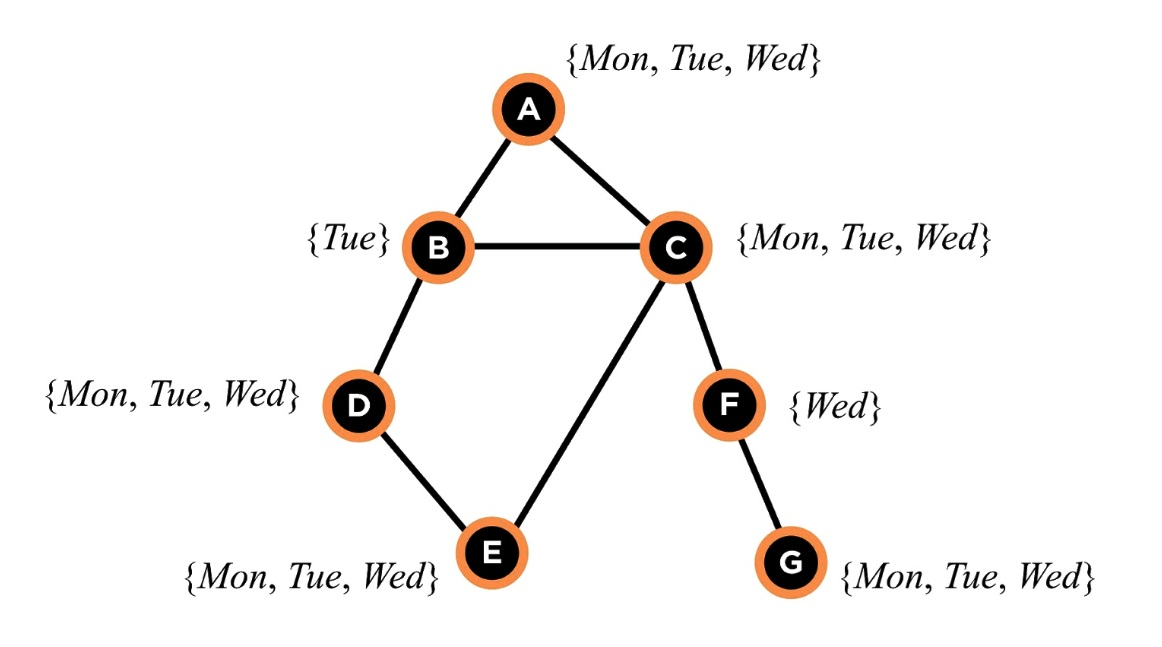
\includegraphics[width=0.8\textwidth]{constraintnetwork.jpg}
\end{figure}

Execute o algoritmo implementado pela função \texttt{order\_domain\_values(self, var, assignment)} para a variável \( C \) e o domínio \{Mon, Tue, Wed\}. Qual será a ordem dos valores no domínio de \( C \) após a execução do algoritmo? 

\section*{Questão 11}

Após aplicar consistência de arcos a todo o problema, quais serão os domínios resultantes para as variáveis \( C \), \( D \) e \( E \)?

\begin{enumerate}
    \item O domínio de \( C \) é \{Mon\}, o domínio de \( D \) é \{Mon, Wed\}, o domínio de \( E \) é \{Tue, Wed\}
    \item O domínio de \( C \) é \{Mon\}, o domínio de \( D \) é \{Tue\}, o domínio de \( E \) é \{QuWeda\}
    \item O domínio de \( C \) é \{Mon\}, o domínio de \( D \) é \{Wed\}, o domínio de \( E \) é \{Tue\}
    \item O domínio de \( C \) é \{Mon, Tue\}, o domínio de \( D \) é \{Wed\}, o domínio de \( E \) é \{Mon\}
    \item O domínio de \( C \) é \{Mon, Tue, Wed\}, o domínio de \( D \) é \{Seg, Qua\}, o domínio de \( E \) é \{Mon, Ter, Wed\}
    \item O domínio de \( C \) é \{Mon\}, o domínio de \( D \) é \{Mon, Wed\}, o domínio de \( E \) é \{Mon, Tue, Wed\}
\end{enumerate}

\section*{Questão 12}

Quais são os 3 cenários possíveis após a execução do algoritmo de consistência de arcos? O que cada cenário diz sobre o problema?

\section*{Questão 13 (Extra)}

Dê um exemplo de um problema de satisfação de restrições que após a execução do algoritmo de consistencia de arcos não resulta em nenhum domínio vazio e ainda assim não possui solução.

\end{document}
